% !TEX root = ../0-main-LN.tex

\setcounter{chapter}{-1}

\chapter{课程简介}

\section{学什么}

高等数学是大学工科专业必修的数学基础课,通常和{\it 线性代数}、{\it 概率论与数理统计}统称
为{\it 工程数学}。

我们所说的高等数学,在国外一般就叫做{\it 微积分},而且通常分为{\it 一元函数微积分}
和{\it 多元(高维)微积分}两个部分。而国外所说的{\it 高等数学}就是我们说的工程数学。

我们一般认为,微积分诞生于17世纪中叶,当时的两位数学巨匠Newton(1642-1726)和
Leibniz(1646-1716)分别独立创立了微积分的理论,并最终被视为微积分的共同发明人。
但是,我们必须认识到的是,一门系统、复杂的理论,不可能仅仅是极个别人的创造。
正如Newton的名言,“{\it If I have seen further, it is by standing on 
the shoulders of giants.}”,在两位大师生前和生后,众多杰出的数学家都为微积分
理论的发展作出了贡献,其中既包括起到奠基作用的Fermat(1607-1665)、Barrow(1630-1677)、
Descartes(1596-1650)%、Huygens(1629-1695)、Wallis(1616-1703)
,也包括使之不断趋于严谨和完善的Cauchy(1789-1857)、D. Bernoulli(1700-1782)、
Lagrange(1736-1913)、Weierstrass(1815-1897)、
Taylor(1685-1731)、Euler(1707-1783)、d'Alembert(1717-1783)
%、Laplace(1749-1827)等
%、Agnesi(1718-1799)
,还有进一步将其发展为更深刻、全面的{\kaishu (数学)分析学}
\ps{分析学和几何学、代数学并称现代数学的三大分支,三者各自拥有庞大的理论体系,
在它们的交汇处诞生了众多重要而又生机勃勃的数学前沿分支}
的
Dirichlet(1805-1859)、Riemann(1826-1866)、Cantor(1845-1918)、
Lebesgue(1875-1941)、
Fourier(1772-1837)等。今天我们所学习的微积分,虽然只是分析学
的基础部分,但要说其中融汇了300多年来众多近现代数学家的杰出成就,是绝对实至名归的。

% \begin{figure}[htbp]
% 	\centering\scalebox{0.3}{\includegraphics{./images/ch1/AM_architecture.jpg}}
% 	\caption{微积分中的主要概念及其关系\;
% 	({\it 个人整理,仅供参考})}
% % 	\label{图:0.1}
% \end{figure}

% \begin{center}
% 	\scalebox{0.3}{\includegraphics{./images/ch1/AM_architecture.jpg}}
% % 	\ps{上课前画好}
% \end{center}

%\begin{center}
%	\includegraphics[width=0.8\textwidth]{./images/ch1/AM_architecture.jpg}
%	
%	{微积分中的主要概念及其关系\;
%	({\it 个人整理,仅供参考})}
%\end{center}

%\begin{center}
%	\includegraphics[width=0.8\textwidth]{./images/%ch1/AM_architecture.jpg}
	%\caption{微积分中的主要概念及其关系}
%\end{center}

\begin{figure}[htbp]
	\centering
	\includegraphics[width=0.8\textwidth]{./images/ch00/AM_architecture.jpg}
	\caption{微积分中的主要概念及其关系\\ ({\it 个人整理,仅供参考})}
\end{figure}

\begin{itemize}
	  \item {\bf 微积分(Calculus)} \hfill from Wikipedia
	\begin{itemize}
	  \item Latin: {\it a small stone used for counting}  
	  \item {\it a branch of mathematics focused on
	  \underline{limits},\underline{functions},
	  \underline{derivatives},\underline{integrals}, and \underline{infinite series} }
  	  \item {\it widespread application in \underline{science},
  	  \underline{economics}, and \underline{engineering}} 
	  \item {\it constitues a major part of modern mathematics}
	  \item {\it 微}的意思是很小的东西,如微生物,{\it 积}就是加起来的意思,
	  {\it 积分}的意思就是把极小的东西加起来。微,是积的相反。 
	\end{itemize}
	\item {\bf John von Neumann} ({\small\it The Mathematician, 1947})
	\begin{itemize}
	  \item {\it The calculus was the \underline{first achievement} of modern
	  mathematics, and it is difficult to overestimate its importance.}
	\end{itemize} 
\end{itemize}

\section{为什么学}

微积分为什么如此重要,毫无疑问,与其在众多领域的应用密不可分,甚至可以说,
在其中绝大多数的问题中,微积分的作用是无可替代的。任何一门工科类的专业课程,
只要涉及与连续运动(变化)相关的问题,都不可避免地会以微积分作为其预备知识,
或者说,将这些课程视为微积分的应用也不为过。

当然,微积分不总是“美丽”的,因为它的美可能不是那么显而易见。我们很难用一两句话
来描述,微积分到底有什么用?它美在哪里?但是,一旦你理解了微积分背后的深刻思想,
开始能够将其应用于解决一些实际问题,或者通过它理解一些最前沿的科技成就时,
你一定会对它的美产生深深地赞叹,也许那时,再回头来看微积分的重要性也就不言而喻了。

学习微积分的过程也许会有些枯燥甚至痛苦\ps{“从前有棵树,叫高数,上面挂了很多人”}
,但它无疑是值得的,能够从看似单调痛苦的过程中领略数学的美丽,发现它的深刻与强大,
也是它作为“{\it 大学第一课}”\ps{无论从体量、难度还是学习的先后来看}所期望带给
大家的体验。

\begin{shaded}
	{\bf 知乎:学数学有什么好处?我们为什么要学数学?}
	\begin{itemize}
	  \item Engles:{\it 数学是一门研究现实世界的数量关系和空间形式的科学。}数学具有:
	  抽象性、精确性和应用的广泛性
	  \item Marx:{\it 一种科学只有在成功运用数学时,才算达到了真正完善的地步。}
	  \item Galileo:{\it “数学符号就是上帝用来书写自然这一伟大著作的统一语言,
	  不了解这些文字就不可能懂得自然的统一语言,只有用数学概念和公式所表达的物理世界
	  的性质才可认识……”}
	  \item Gauss:{数学是科学的女王}
	  \item 韩寒:{\it
	  我们生活中用到的数学估计到小学三年级就已经够用了。}然而在之后我们多年来学习的数学,
	  实际上塑造了我们一种理性的、条理的、系统化的思维方式。这种思维方式在我们解决自己
	  一生中遇到的诸多问题时,都有非常重要的作用。比如慎密的思考、分类的思想、排序的思想等。
	  很多东西其实都带有学习数学这个过程产生的影响,只是由于其作用方式非常隐晦,
	  也不容易被追溯其源头,我们平时不容易注意到罢了。
	  \item 王小波:{\it 我上大学时,有一次我的数学教授在课堂上讲到:我现在所教的数学,
	  你们也许一声都用不到,但我还要教,因为这些知识是好的,应该让你们知道。”}
	\end{itemize}

	{\bf 其他的说法:}
	\begin{itemize}
	  \item {\bf 数学的三大功能}
	  \begin{enumerate}
	    \item 为学习其他知识(课程)提供数学工具
	    \item 培养理性思维
	    \item 弘扬数学文化
	  \end{enumerate}
	  \item {\bf 数学素质}
	  \begin{enumerate}
	    \item 从实际问题抽象出数学模型的能力
	    \item 计算与分析的能力
	    \item 了解和使用现代数学语言和符号的能力
	    \item 使用数学软件学习和应用数学的能力
	  \end{enumerate}
	\end{itemize}
\end{shaded}

\begin{itemize}
	\setlength{\itemindent}{1cm}
	\item {用通用简洁的方式来表达自然规律;}
	\item {提供一些问题的分析手段;}
	\item {提供认识世界的一种模式;}
	\item {了解自己的智力水平。}
\end{itemize}

\section{怎么学}

\begin{itemize}
	\item {\bf 参考资料}
  	\begin{enumerate}
		\item {\bf 教材与必备资料}
	  	\begin{itemize}
	  	  \item {同济大学数学系,高等数学(第七版,上、下),
	  	  高等教育出版社,2014,北京}\ps{简称:\b 同济}  
	  	  \dotfill{\kaishu\b 考研指定教材,建议人手一套}
	  	  \item {朱健民 等,高等数学(第二版,上、下),
	  	  高等教育出版社,2015,北京}
	  	  \ps{简称:\b KD教材} 
	      \item {李建平 等,高等数学典型例题
	      与解法(上、下),国防科技大学出版社,2009,}
	      {长沙}
	      \ps{简称:\b 辅导书} 
	  	\end{itemize}
  		\item {\bf 参考书} 
  		\begin{itemize}
	    	\item 菲赫金哥尔茨,微积分学教程(第一至三卷),
	    	第8版,高等教育出版社,2006,北京
	    	\dotfill{\it\b 读不懂不必勉强,它回答不了的微积分问题
	    	大学阶段你肯定碰不到} 
	    	\item James Stewart, Calculus(7th eds.)(影印版,上、下册),高等教育出版社,2014,北京
	    	\dotfill{\it\b 大部头,但绝对浅显易懂}
	    	\item 斯蒂芬.弗莱彻.休森,数学桥,上海科技出版社,2010,上海
	    	\ldots\dotfill{\it\b 值得常常拿出来读的数学书,一遍绝对不够} 
	    	\item William Dunham,微积分的历程——从牛顿到勒贝格,人民邮电出版社,2011,北京
	    	\dotfill{\it\b 了解微积分的历史,能够更好地理解其中深刻的思想} 
  		\end{itemize}
  		\item {\bf 在线资源}
  		\begin{itemize}
  		  \item {朱健民,高等数学(一-五),中国大学MOOC},
  		  \url{http://www.icourse163.org/course/NUDT-9004}
  		  \ps{简称:\b MOOC}\ldots
  		  \dotfill{\it\b 缺课或者课上没听懂,可以它补补课}
  		  \item underline{李建平\,等,高等数学典型例题与解法(一、二),中国大学MOOC}
  		  \url{http://www.icourse163.org/course/NUDT-1001979006}
  		  \ldots\dotfill{\kaishu\b 与KD教材配套的习题课}
  		  \item 闫浩,高等数学习题课,学堂在线
  		  \url{https://xuetangx.com/courses/course-v1:BUPT+3412113011+2017_T2/about}
  		  \dotfill{\it\b 讲得很棒,这老师原来是清华的}
   		  \item 李建平\,等,微积分CAP,中国大学MOOC
  		  \url{http://www.icourse163.org/course/NUDT-1001626005}
   		  \dotfill{\it\b 高中没学好,来这补一补}
		\end{itemize} 
		\item {\bf 扩展阅读}\dotfill{\it\b 读一些课外书,让学习显得不那么枯燥}
		\begin{itemize}
		  \item 基斯.德夫林,数学思维导论,人民邮电出版社,2016,北京
		  \item G.波利亚,怎样解题:数学思维的新方法,上海科技教育出版社,2011,上海
		  \item 李学数,数学与数学家的故事(1-5),上海科学技术出版社,2015,上海
		  \item 塞德里克·维拉尼\,等,一个定理的诞生:我与菲尔茨奖的一千个日夜,人民邮电出版社,2016,北京
		  \item 春日真人,庞家莱猜想:追寻宇宙的形状,人民邮电出版社,2015,北京
		  \item 蒂莫西.高尔斯,数学,译林出版社,2014,南京
		  \item 吴军,数学之美,人民邮电出版社,2016,北京
		  \item 李建平,漫谈数学与军事,中国大学MOOC
		\end{itemize}
	\end{enumerate}
	\item {\bf 学习方法}
	\begin{enumerate}
	  \item {\bf 预习:}课前3-5分钟,快速翻阅教材,浏览本讲内容梗概,
	  标记出新的名词和例题,试着理解其大概意思,确保听课时心中有数;
	  \item {\bf 听课:}抓住关键思路,卡住了或者有疑点立即举手问,
	  简要记笔记\ps{推荐:\b 康奈尔笔记法},重点记思路和书本上没有的内容
	  \item {\bf 复习:}要么读教材,要么读笔记,也可以先作习题,搞不定
	  再回来翻书查笔记,重在理清思路\ps{重要概念,典型问题,典型方法},
	  消化细节,肯花时间才有好的效果
	  \item {\bf 练习:}作业之外,有选择地作题,学习也是个熟能生巧的过程,
	  提高效率是关键\\
	  G.Polya:{\it 我们的任何一门学问都由知识和技能组成。如果你对初等或高等数学的研究工作
	  的确有真正的经验的话,那么你对下述这一点将毫不怀疑:在数学中,技能比仅仅掌握
	  一些知识要重要得多。什么是技能呢?数学技能就是解题能力——不仅能解决一般的问题,
	  而且能解决需要某种程度的独立思考、判断力、独创性和想象力的问题}
	  \item {\bf 思考:}多琢磨,让知识点在大脑中结成网络,融会贯通,
	  会提问是思考能力的体现\ps{Einstein:提出一个问题往往比解决一个问题更重要!}
	\end{enumerate}
\end{itemize}

一种好的学习、思考路径:
{\it What$\to$How$\to$Why$\to$Why not$\to$What if}

\section{几点要求}
\begin{itemize}
	\item {\bf 课堂:安静!安静!!安静!!!}
	尊重他人学习的权利,安排好自己的时间
	
	{\bf - No to}
	  \begin{itemize}
	    \item Chatting
	    \item zZZ\ldots
	    \item anything noisy
	    \item \ldots
	  \end{itemize}
	{\bf - Yes to}
  \begin{itemize}
    \item listen to me
    \item discuss {\bf with me}
    \item do sth. you like {\bf quietly}
    \item zzz\ldots
    \item leave/enter the classroom {\bf quietly}
    \item \ldots
  \end{itemize}
  \item {\bf 作业}
  \begin{figure}[h]
  	\begin{center}
  		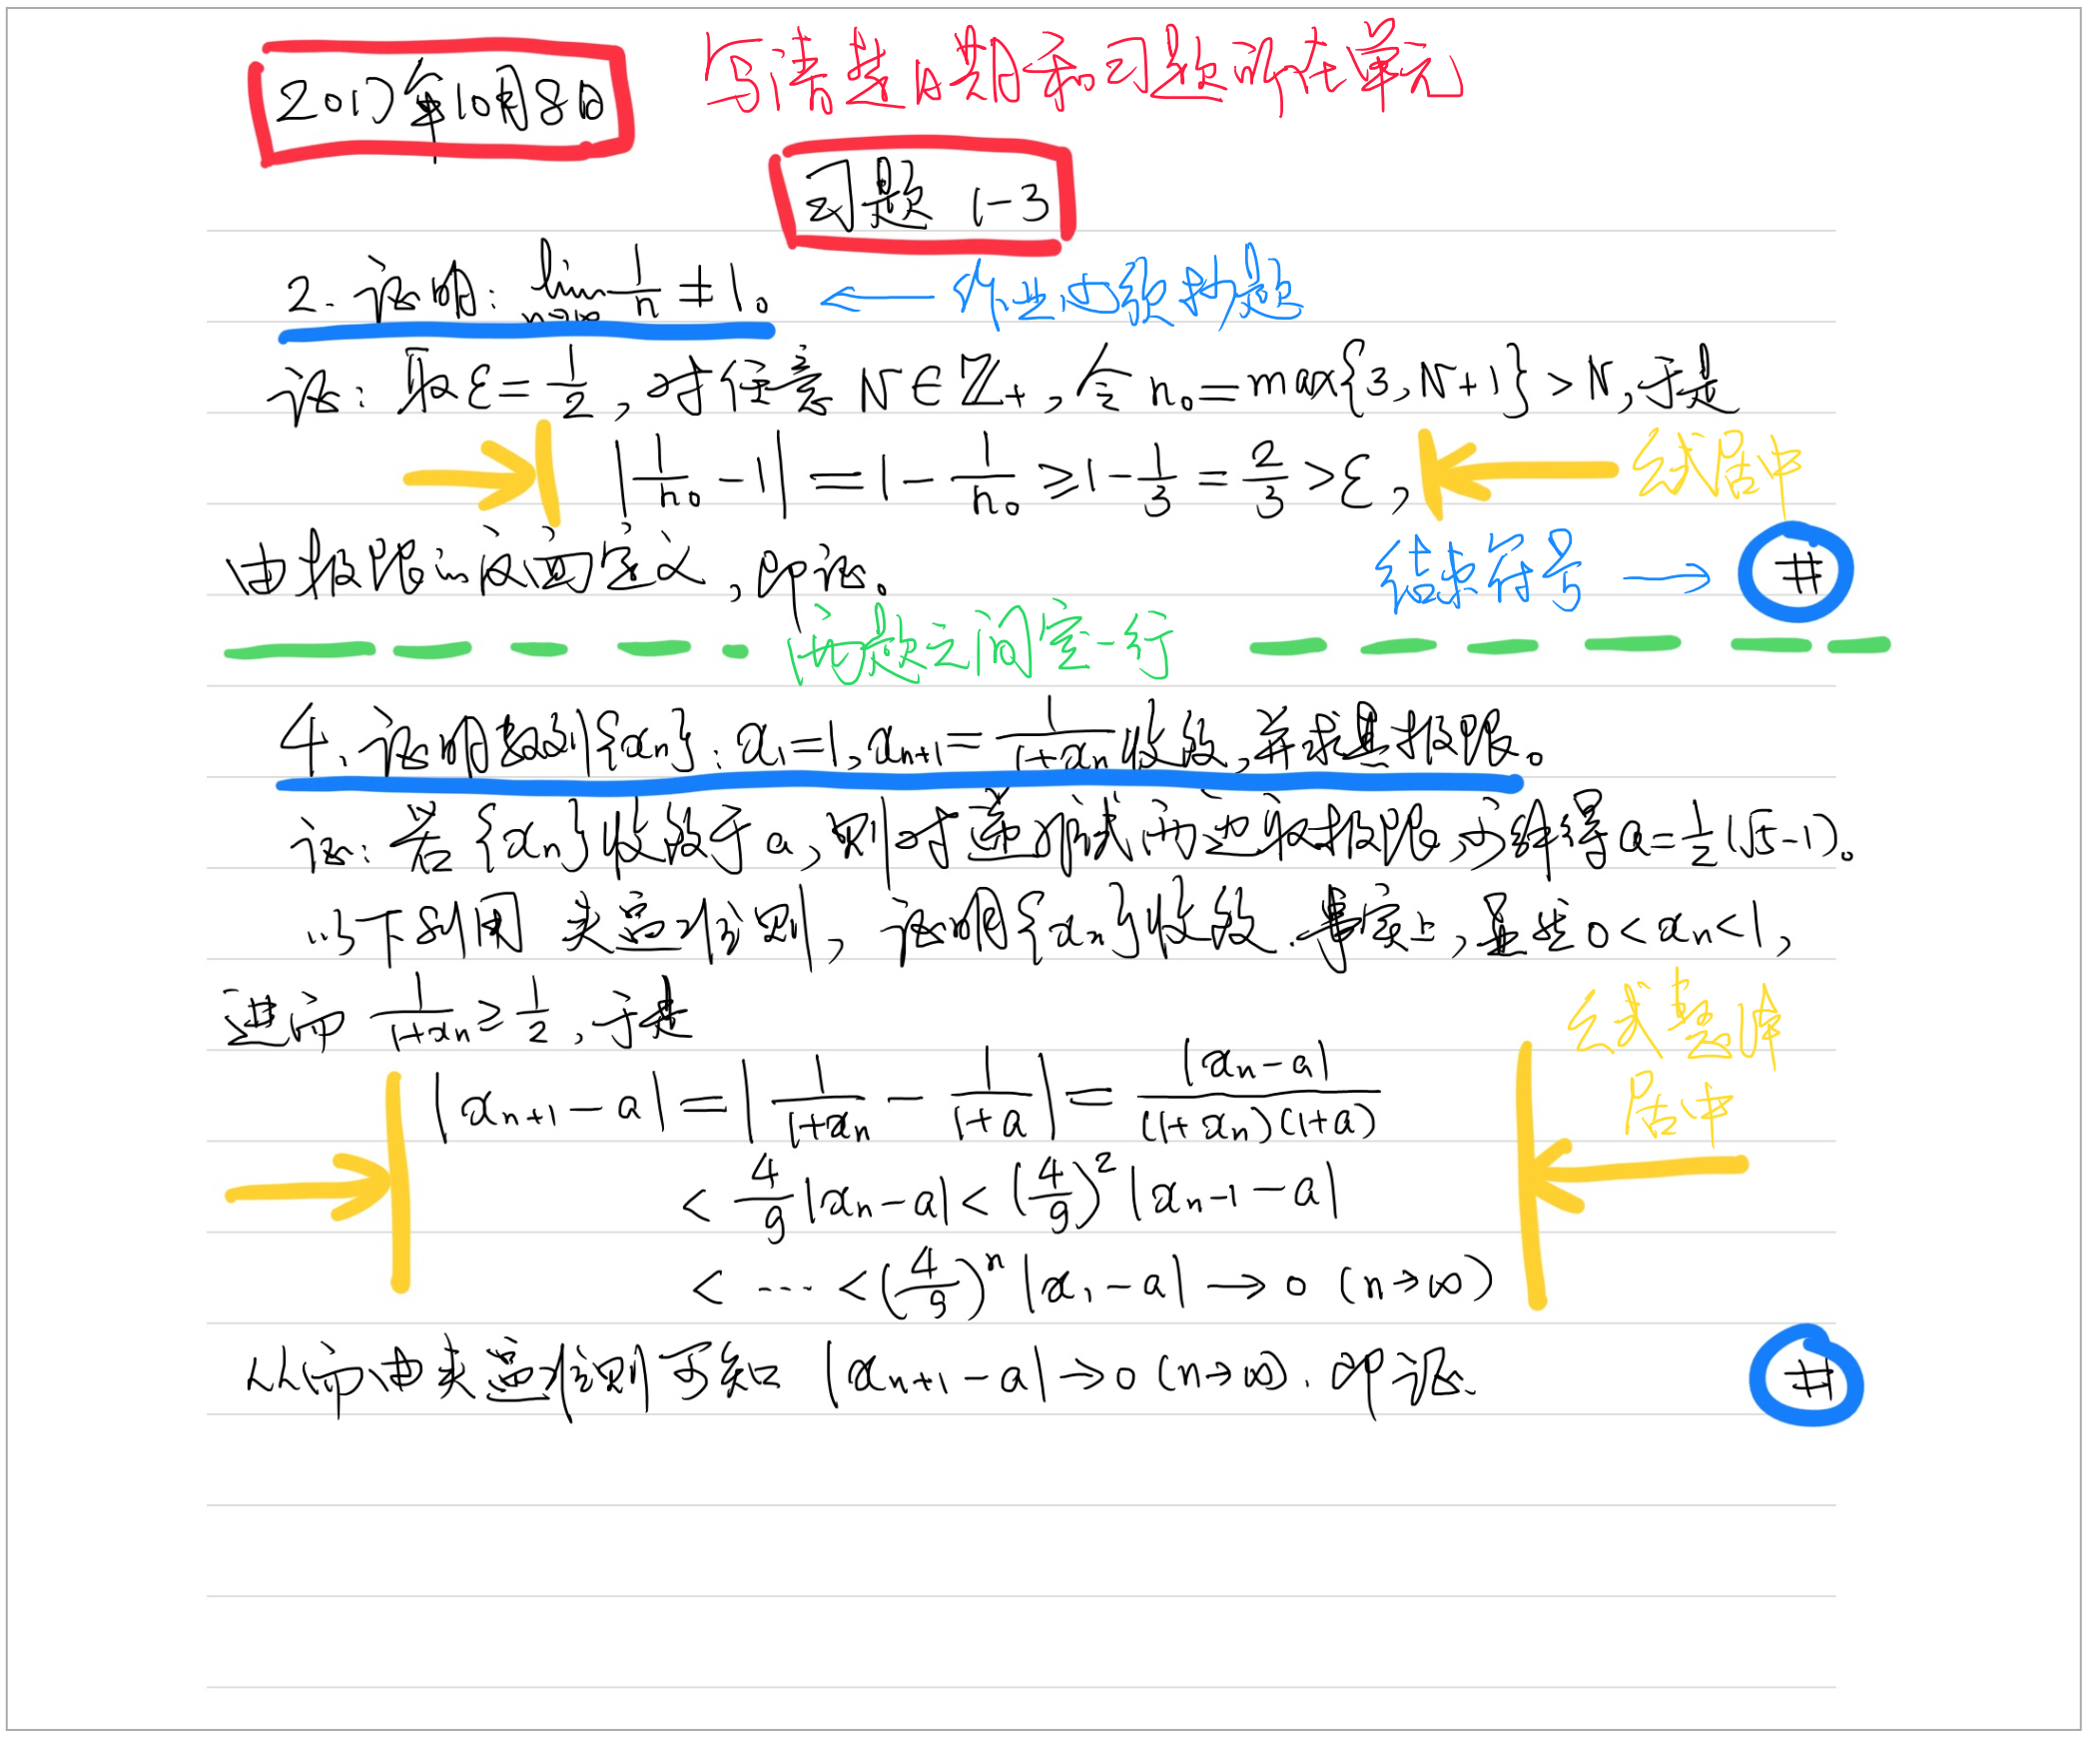
\includegraphics[width=0.95\textwidth]{./images/Ch00/hw-sample.jpg}
  		\caption{作业参考格式\\ (以黑色字体为准,彩色部分为格式说明)}
  		\label{fig:0.2}
  	\end{center}
  \end{figure}
  \begin{itemize}
    \item 书写规范
    \begin{enumerate}
      \item 写清楚作业日期(对应讲课的日期)和习题所在单元;
      \item 作业必须抄题,写清楚题号;
	  \item 解题过程以“证:”或“解:”开始,以$\#$号结束;
	  \item 公式整体居中书写;
	  \item 无论大题小题,两题之间空一行;
	  \item 不允许使用铅笔、红笔书写作业,可以用铅笔画图;
	  \item 作业本不许分栏使用;
	  \item 文字、符号书写清晰规范,尽量少涂改。
    \end{enumerate}    
    \item 不要做“复印机”!
    \item 及时订正错误,补上缺漏。
  \end{itemize}
	\item {\bf 答疑}
	  \begin{itemize}
	    \item 每周一次面对面答疑,1-2小时;
	    \item 提问题的能力不完全是天生的,脸皮要厚一点!
	    \item 综合利用各种手段(微信、网站、邮件、\ldots)
	  \end{itemize}
% 	  \item {\bf 从善如流}
\end{itemize}

\section{关于考试}

%以下是2017-2018学年开始实施的“{\it 新政}”:

考试分为{\it 形成性考试}和{\it 终结性考试}两个部分,两部分成绩按照$40\%$和$60\%$的比例综合
得到最终的课程期末成绩。

每学期末设一次终结性考试,采用闭卷笔试形式。{\baa 终结性考试不及格,
则课程成绩不合格!}

每学期的形成性考试分为四个部分,一是{\it 平时作业和表现}成绩,占$10\%$,剩下的为三次
{\it 单元测试}成绩,各占$10\%$。

单元测验的形式为笔试或网络测试,具体待定。

\newpage

\begin{ext}
	\begin{center}
		\bf 课后作业
	\end{center}
	
	%{\b\it 说明:作业必须写明题目所在章节、页码、题号;如非特别说明,
	%所有题目必须抄题;两道题之间空一行;未作或作错的题目讲评后务必及时订正。}
	
	\begin{enumerate}
	  \item 加老师的QQ:20847517,发送自己的姓名作为验证信息;
	  \item 登录中国大学MOOC网站:\href{http://www.icourses.cn/imooc/}
	  {http://www.icourses.cn/imooc/}
	  ,完成以下任务:
	  \begin{enumerate}[(1)]
	  	\item 注册中国大学MOOC账号,将“学号、姓名、账号”告知课代表统一登记;
	  	\item 通过链接:\href{http://www.icourse163.org/spoc/course/NUDT-328003}
	  	{http://www.icourse163.org/spoc/course/NUDT-328003}加入我校开设的SPOC课程《高等数学(一)》
	  	\ps{本课程所有的单元测验都将通过SPOC课程进行,
	  	后续还将开设《高等数学(二)》至《高等数学(五)》}
	  	,课程密码为:nudt742340;
	  	\item 搜索并加入我校自己开设的MOOC课程:
	  	\href{https://www.icourse163.org/course/NUDT-9004}
	  	{《高等数学(一)》}、
	  	\href{https://www.icourse163.org/course/NUDT-1001616011}
	  	{《高等数学典型例题与解法(一)》}
	  	及
	  	\href{https://www.icourse163.org/course/NUDT-1002011022}
	  	{《漫谈数学与军事》}。
	  \end{enumerate}
	  \item 写一篇短文,内容及要求如下:
	  \begin{enumerate}[(1)]
	    \item 你的个人介绍,请务必包含如下信息:姓名、性别、年龄、籍贯、
	    中学母校的名字、你的高考总成绩(以及当地的满分)、
	    你的高考数学成绩(以及当地的满分);
	    \item 你的兴趣爱好、特长,或者说,你觉得自己有什么与众不同之处;
	    \item 你学习数学的体会,例如:喜欢什么样的数学,不喜欢什么样的数学?
	    有什么你个人觉得比较好的学习方法、成功的经验,或者有趣的经历
	    (最好与数学有关)?
	    \item 你对大学的课堂有什么期待?怎么样的教与学会对你更有帮助?
	    对老师有什么要求或者建议?
	    \item 请至少推荐一本(部、套)你喜欢的书、电影或者其他任何可以
	    通过公共渠道获取到的资料(例如:网站、软件、APP、\ldots),说说推荐的理由;
	    \item 其他任何你认为值得(可以)与老师交流的东西,比如你想问我什么
	    都可以问;
	    \item 除第一条必须包含外,其余内容可自由取舍;
	    \item 篇幅不少于半页活页纸(A4或16K),不多于两页(一张的正反面)。
	  \end{enumerate}
	  \item 自行了解学习康奈尔笔记法(本章附录);
	  \item 自行阅读李开复博士的《给未来的你》(稍后会发在课程的QQ群内);
	  \item 自行完成课前自测题(稍后会发在课程的QQ群内),不必上交。
	\end{enumerate}
\end{ext}

\newpage

\section*{附录:Cornell Note-Taking System}
\addcontentsline{toc}{section}{附录:Cornell Note-Taking System}

\thispagestyle{empty}

Cornell Note-Taking System,或康奈尔笔记法(5R笔记法),
适用于一切依赖讲授或自学的学习过程,特别是对于听课笔记堪称首选。
该方法的重点是记与学、思考与运用的结合,以及将笔记的记录与完善
作为学习的过程载体。最终完成的笔记类似于下图:

\begin{figure}[h]
	\centering
	\begin{subfigure}[t]{0.45\textwidth}
		\centering
		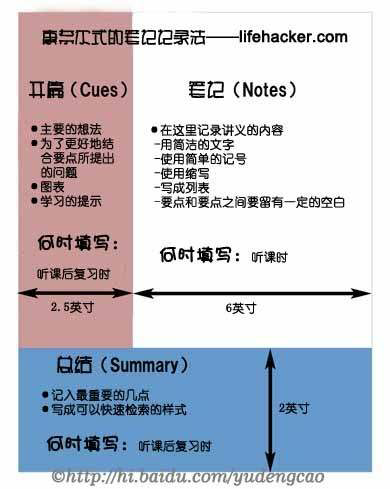
\includegraphics[width=\textwidth]{./images/Ch00/Cornell-NTS/NTS-CH.jpg}
		\caption{布局}\label{fig:5R-1}
	\end{subfigure}
	\begin{subfigure}[t]{0.45\textwidth}
		\centering
		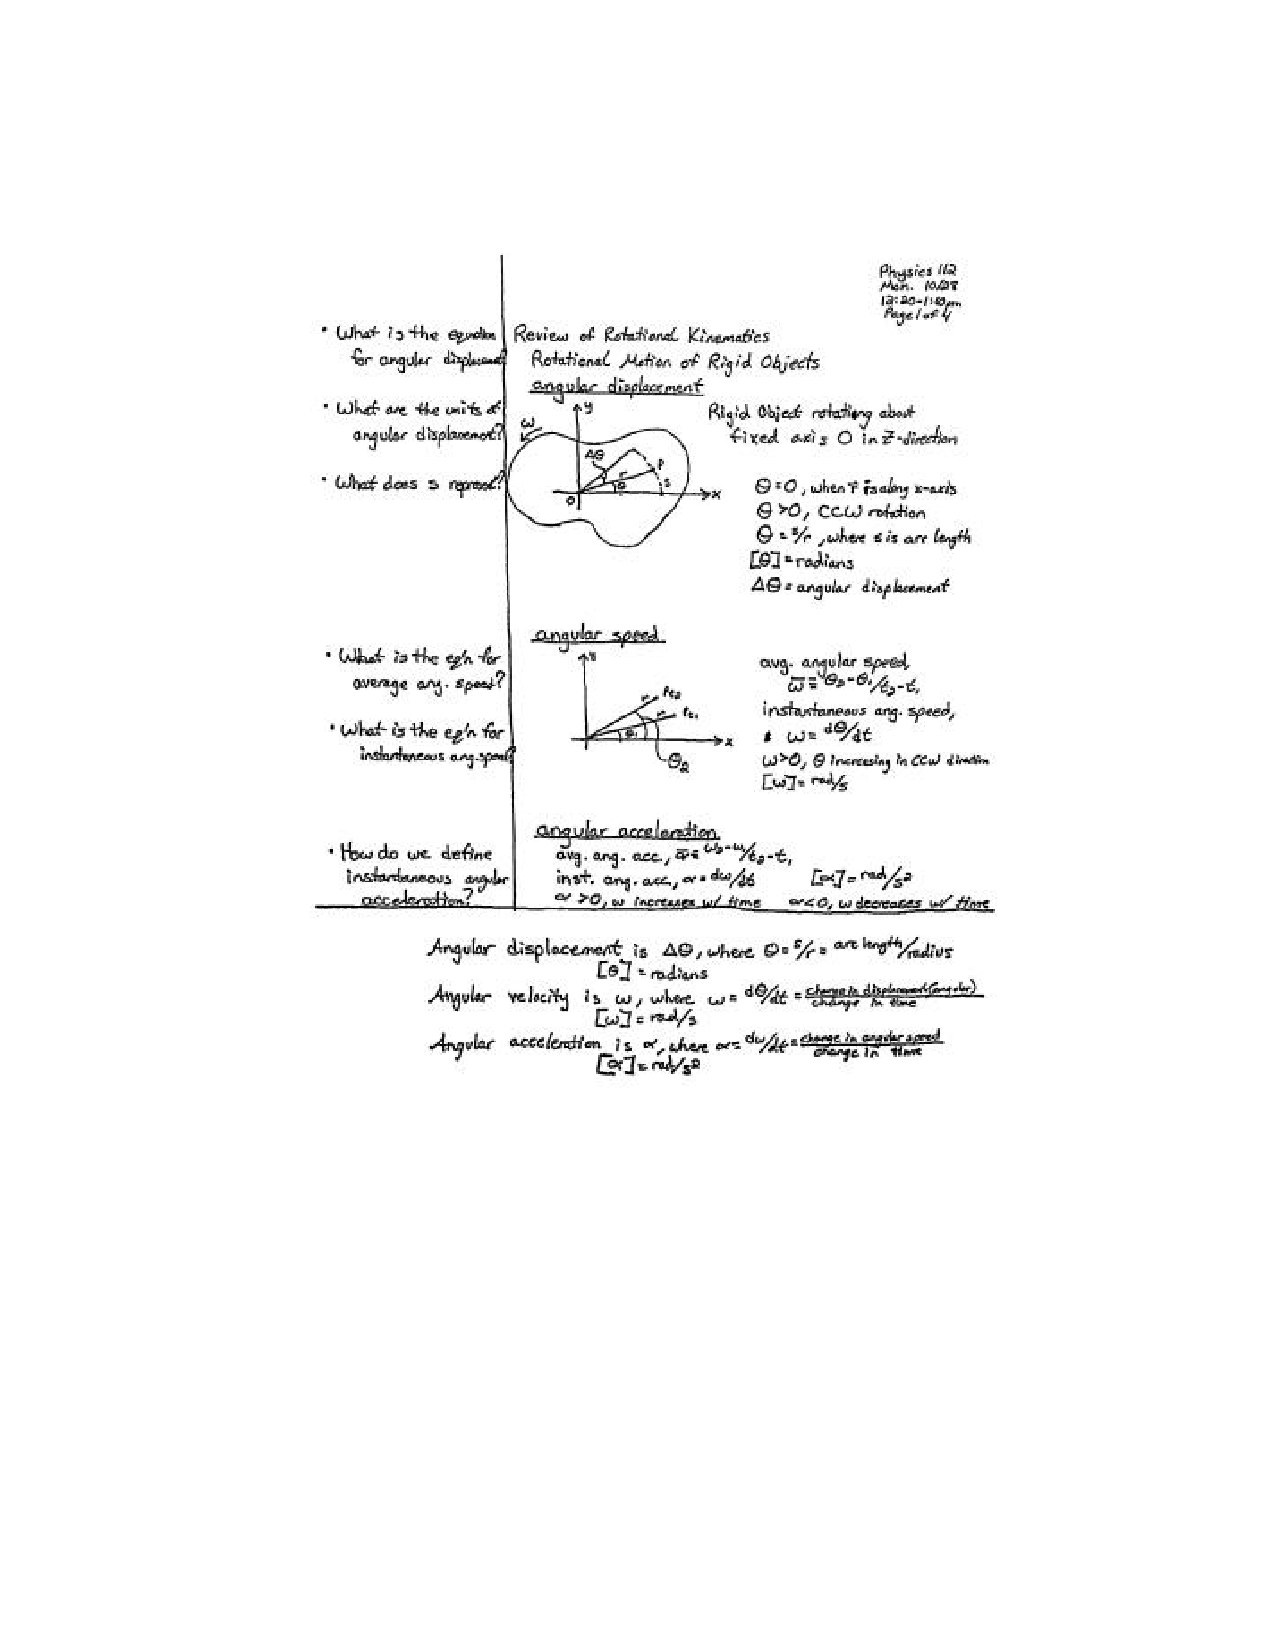
\includegraphics[width=\textwidth]{./images/Ch00/Cornell-NTS/exCNTS.pdf}
		\caption{示例}\label{fig:5R-2}
	\end{subfigure}
	\caption{5R笔记法}\label{fig:5R}
\end{figure}
	
笔记的行程过程可以分为所谓的{\bf 5R}:

\begin{enumerate}[Step1]
  \setlength{\itemindent}{1cm}
  \setlength{\topsep}{0pt}
  \item {\it 记录(Record):}在听讲或阅读过程中,
  在主栏(将笔记本的一页分为左大右小两部分,
  左侧为主栏,右侧为副栏)内尽量多记有意义的论据、概念等讲课内容。
  \item {\it 简化(Reduce):}下课以后,尽可能及早将这些论据、概念简明扼要地概括(简化)
  在回忆栏,即副栏。
  \item {\it 背诵(Recite):}把主栏遮住,只用回忆栏中的摘记提示,
  尽量完满地叙述课堂上讲过的内容。
  \item {\it 思考(Reflect):}将自己的听课随感、意见、经验体会之类的内容,
  与讲课内容区分开,写在卡片或笔记本的某一单独部分,加上标题和索引,
  编制成提纲、摘要,分成类目。并随时归档。
  \item {\it 复习(Review):}每周花十分钟左右时间,快速复习笔记,主要是先看回忆栏,
  适当看主栏。
\end{enumerate}

在课本、参考书原文的旁边加上各种符号(如直线、双线、黑点、圆圈、
曲线、箭头、红线、蓝线、三角、方框、着重号、惊叹号、问号等等),便于找出重点,
加深印象,或提出质疑。什么符号代表什么意思,自己掌握即可,但最好形成一套比较
稳定的符号系统。这种方法特别适合于自学笔记和预习笔记。

操作时注意以下一些准则:
{\it 读完后再做记号,要非常善于选择,用自己的话进行注记,
形式和过程力求简洁、迅速、整齐}

笔记的加工:{\it 忆$\to$补$\to$改$\to$编$\to$分$\to$舍$\to$记}	

\newpage

\begin{figure}[t]
	\centering
	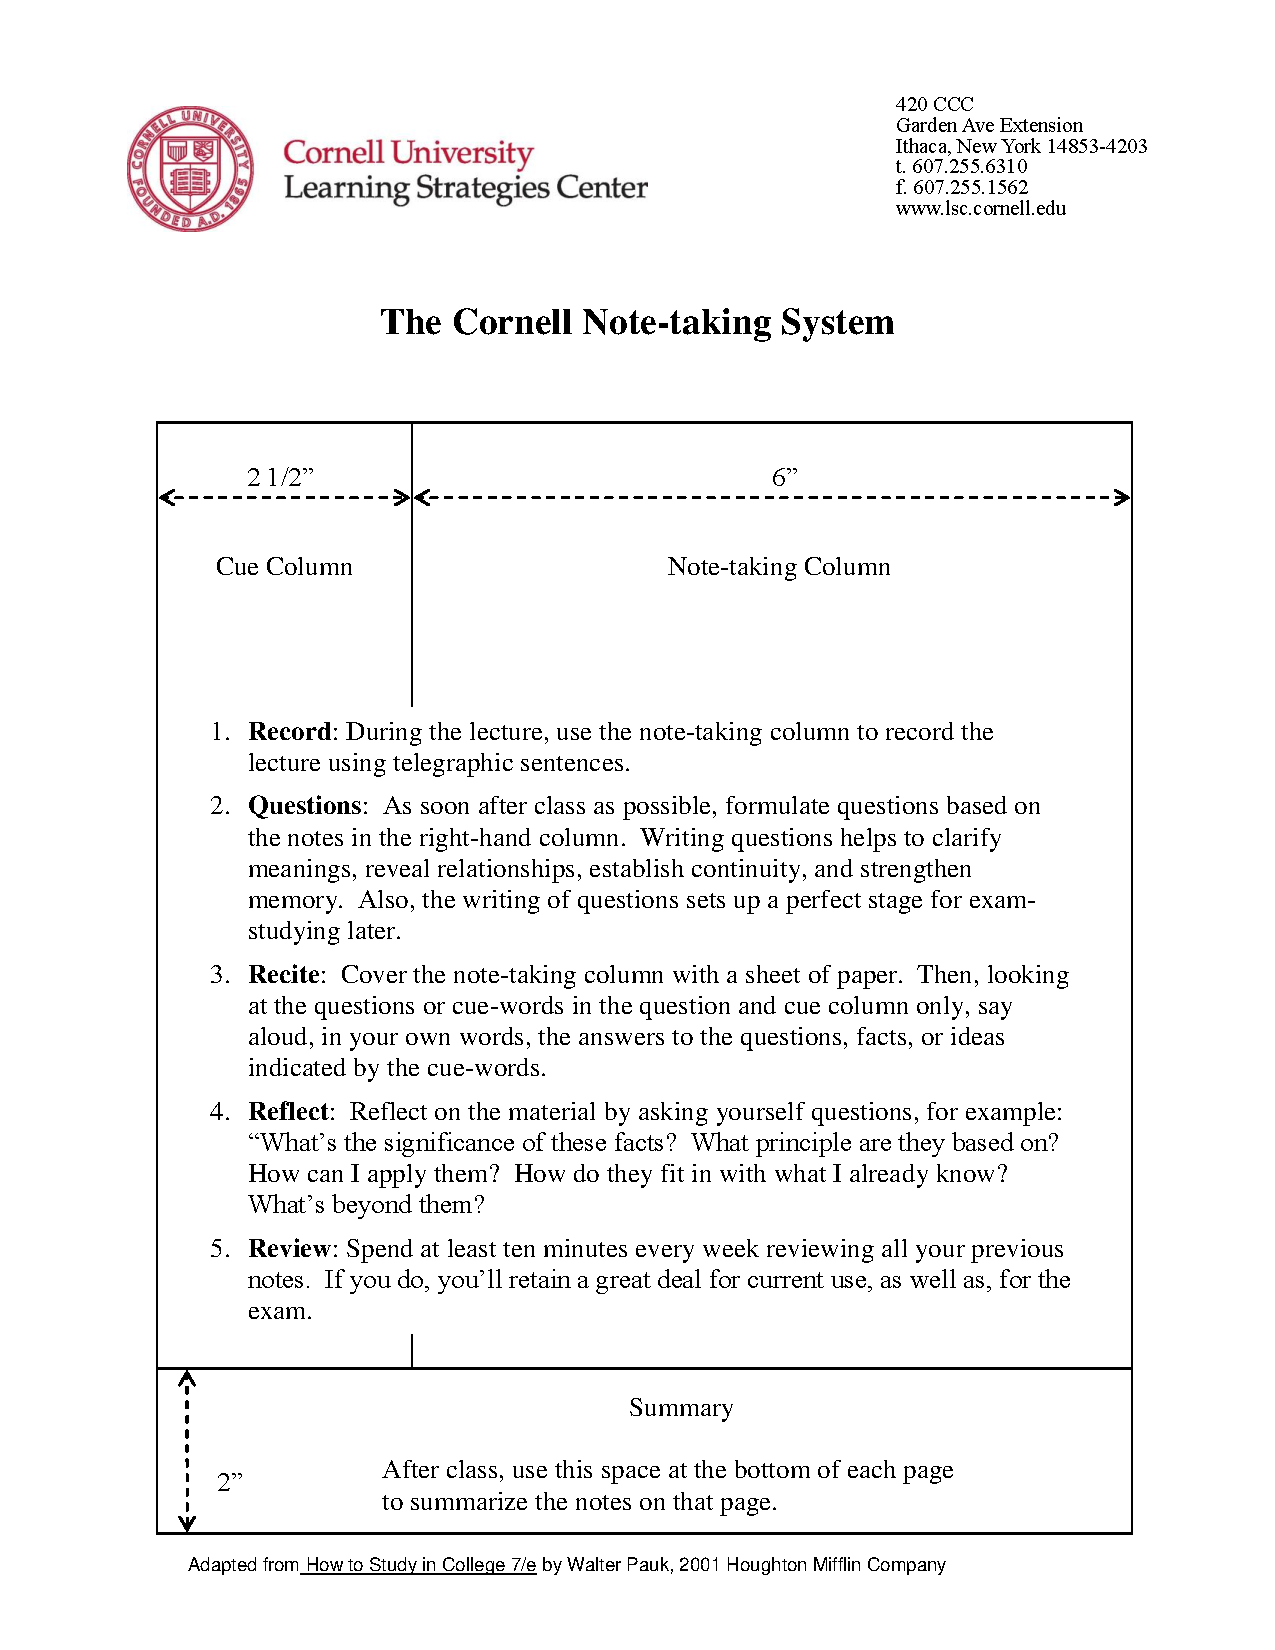
\includegraphics[width=\textwidth]{./Images/Ch00/Cornell-NTS/Cornell-NoteTaking-System.pdf}
	\caption{Cornell Note-taking System (from: \href{http://lsc.cornell.edu/notes.html}{http://lsc.cornell.edu/})}
\end{figure}

\thispagestyle{empty}